Das bereits bekannte Eisen-Kohlenstoff-Diagramm nimmt eine derart lange Abkühlphase an, dass sich durch Versetzungen aber
vor allem auch durch Diffusion der Fremdatome Gitterstrukturen thermodynamisch ausgleichen können. Versetzungen geschehen
allerdings um ein vielfaches schneller. Bei der Umwandlung vom krz-Austenit zum kfz- Technisch relevante Stähle
haben Kohlenstoffkonzentrationen bis 2,06\% was der maximalen Löslichkeit von C in Austenit (bei etwa \SI[]{1150}{\celsius})
entspricht.

Durch höhere Abkühlraten aus dem Austenit heraus können allerdings bestimmte Gefügeungleichgewichte forciert und in ihrem
Istzustand eingefrohren werden. Hierdurch wiederum lassen sich Parameter wie Härtegrad, Zähigkeit und dergleichen mehr
steuern.
\begin{wrapfigure}{r}{0.5\textwidth}
    \vspace{-10pt}
    \centering
    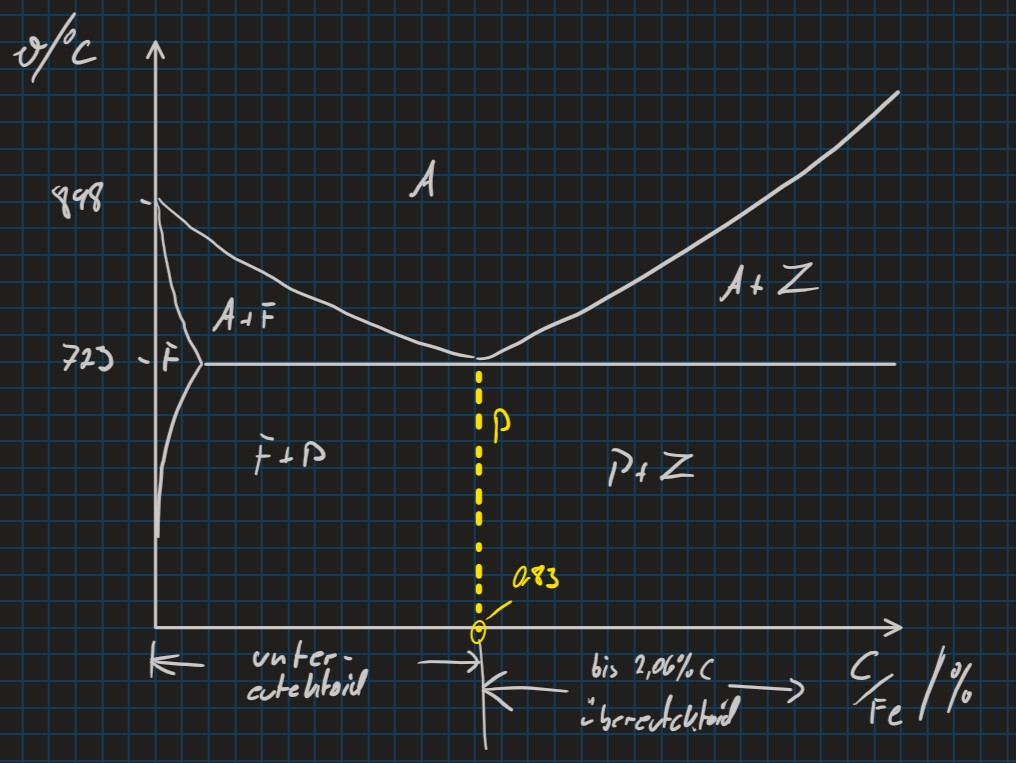
\includegraphics[width=0.5\textwidth]{entries/8/eutektoid.jpg}
    \caption{\textbf{A}: Austenit, \textbf{F}: Ferrit, \textbf{P}: Perlit, \textbf{Z}: Zementit. Das kleine Eutektikum (aka Eutektoid) ist der Bereich von 0 bis 2,06\% C Gehalt.}
    \label{fig:eutekt}
\end{wrapfigure}
Der besonders harte Martensit etwa kann nur hergestellt werden, wenn bei der Umwandlung vom kubisch-flächenzentrierten
Austenit zum kubisch-raumzentrierten Ferrit dem Kohlenstoff keine Zeit gelassen wird aus den Gittern hinaus zu diffundieren.
In Folge bleibt der Kohlenstoff im krz zwangsgelößt und verzerrt selbiges derart, dass es über mehrere Einheitszellen hinweg
keine größeren Gleitebenen mehr gibt. Welche Abkühlraten oder auch Haltezeiten es bedarf um jeweilige Gefügekonfigurationen
zu erreichen lassen sich aus einem Zeit-Temperatur-Umwandlungsdiagramm oder englisch Time-Temperature-Transformation Diagram
(kurz ZTU bzw. TTT) ablesen. Im Prinzip ist das ZTU eine Erweiterung des Eisen-Kohlenstoff-Diagramms um eine dritte Dimension
- die Abkühlrate.
Nun können und werden in das ZTU Linien eingezeichnet, die wie Anleitungen zur Herstellung von Stählen ganz bestimmter
Härtegrade etc. gelesen werden können.

Doch stop! Woher kommt der Stahl? Fällt ja nicht einfach vom Himmel \footnote[1]{Streng genommen trifft das auf Bestandteile
des Stahls nicht immer zu. Der Dolch der als Grabbeigabe Tutanchamuns diente wurde etwa aus von Meteoriten gewonnenem Eisen
geschmieded. Mindblowing? Ziemlich. Dennoch war es zu Frühzeiten nicht unüblich Meteoritengestein als Eisenquelle zu nutzen.
Allerdings waren die Menschen sich damals nicht unbedingt bewusst, dass es sich um einen aus dem Himmel gefallenen Stein handelt.}.
Der Grundbestandteil Eisen wird mit großem Aufwand in Form von Magnetit (Magneteisenstein, \(Fe_3 O_4\)), Hämatit
(Roteisenstein, \(Fe_2 O_3\)), Limonit (Brauneisenstein, \(2Fe_2 O_3 \cdot 3H_2 O\)) und/oder Siderit (Spateisenstein,
\(FeCO_3\)) vor. Da das Erz einerseits in oxidierter Form vorliegt und andererseits nicht frei von Verunreinigungen ist
muss es um es nutzbar zu machen zunächst reduziert und von Beielementen gereinigt werden. Der im Skript beschriebene
Prozess der indirekten Reduktion mittels Kohlenmonoxid ist allerdings etwas verbuggt. Die Summenformeln gehen nicht auf
und zumindest im Abgleich mit externen Quellen werden Zwischenschritte sind unter den Tisch fallen gelassen.
\begin{align}
    &\text{\Romannum{1}} &3Fe_2 O_3 + CO &\rightarrow 2Fe_3 O_4 + CO_2\\
    &\text{\Romannum{2}} &Fe_3 O_4 + CO &\rightarrow 3FeO + CO_2\\
    &\text{\Romannum{3}} &FeO + CO &\rightarrow Fe + CO_2
\end{align}
Zusätzlich ist im Begleitdokument auf Produktseite \(\SI[]{4200}{\frac{kJ}{kg}}Fe\) angegeben. Meiner Recherche zufolge ist
die Reduktion von Eisen eine endotherme Reaktion. Da es mir nicht vergönnt war konkrete Werte zu recherchieren und darüber hinaus meine
Kenntnisse der Chemie bestenfalls dilettantisch sind kann ich nur vermuten, dass der Ofen bzw. sein Inhalt um diese
Wärmemenge (durch die Reaktion) gekühlt wird. Rechnerisch würde das bedeuten, grob über den Daumen gepeilt, dass \(\thicksim \SI[]{48,6}{kW}\)
der aufgewandten Energie rein in die Reaktion geht (\SI[]{1000}{kg} Fe Tagesproduktion).